\documentclass[a4paper, 12pt]{report}		% general format
\usepackage{multicol}
%%%% Charset
\usepackage{cmap}							% make PDF files searchable and copyable
\usepackage{bm}
\usepackage{pdfpages}
\usepackage[utf8x]{inputenc} 				% accept different input encodings
\usepackage[english,russian]{babel}   %% загружает пакет многоязыковой вёрстки
%\usepackage{fontspec}      %% подготавливает загрузку шрифтов Open Type, True Type и др.
%\defaultfontfeatures{Ligatures={TeX},Renderer=Basic}  %% свойства шрифтов по умолчанию
%\setmainfont[Ligatures={TeX,Historic}]{Roboto-Light} %% задаёт основной шрифт документа
%\setsansfont{Roboto-Light}  
\usepackage{float}
%%%% Graphics
%\usepackage[dvipsnames]{xcolor}			% driver-independent color extensions
\usepackage{graphicx}						% enhanced support for graphics
\usepackage{wrapfig}						% produces figures which text can flow around

%%%% Math
\usepackage{amsmath}						% American Mathematical Society (AMS) math facilities
\usepackage{amsfonts}						% fonts from the AMS
\usepackage{amssymb}						% additional math symbols

%%%% Typograpy (don't forget about cm-super)
\usepackage{microtype}						% subliminal refinements towards typographical perfection
\linespread{1.0}							% line spacing
\usepackage[mag=1000, left=2.0cm, right=1.5cm, top=2cm, bottom=2cm, headsep=0.7cm, footskip=1cm]{geometry}
\setlength{\parindent}{0pt}					% we don't want any paragraph indentation
\usepackage{parskip}						% some distance between paragraphs

%%%% Tables
\usepackage{tabularx}						% tables with variable width columns
\usepackage{multirow}						% for tabularx
\usepackage{hhline}							% for tabularx
\usepackage{tabu}
\usepackage{longtable}

%%%% Graph
\usepackage{tikz}							% package for creating graphics programmatically
\usetikzlibrary{arrows}						% edges for tikz

%%%% Other
\usepackage{url}							% verbatim with URL-sensitive line breaks
\usepackage{fancyvrb}						% sophisticated verbatim text (with box)

\usepackage{fancyhdr}
\usepackage{latexsym}
\usepackage{booktabs}
\usepackage{array}

\usepackage{listings}
\usepackage{caption}
\DeclareCaptionFont{white}{\color{white}}
\DeclareCaptionFormat{listing}{\colorbox{gray}{\parbox{\dimexpr\textwidth-1.72\fboxsep\relax}{#1#2#3}}}
\captionsetup[lstlisting]{format=listing,labelfont=white,textfont=white,margin=0pt}
\lstset{language=C,
	basicstyle=\footnotesize,
	keepspaces=true,
	tabsize=4,               
	frame=single,                           % Single frame around code
	rulecolor=\color{black},
	captionpos=b,
	showstringspaces=false,	
	abovecaptionskip=-0.9pt,
	xleftmargin=3.4pt,
	xrightmargin=2.6pt,
	breaklines=true,
	postbreak=\raisebox{0ex}[0ex][0ex]{\ensuremath{\color{black}\hookrightarrow\space}},
	xleftmargin=3.2pt,
	literate={а}{{\selectfont\char224}}1
	{~}{{\textasciitilde}}1
	{б}{{\selectfont\char225}}1
	{в}{{\selectfont\char226}}1
	{г}{{\selectfont\char227}}1
	{д}{{\selectfont\char228}}1
	{е}{{\selectfont\char229}}1
	{ё}{{\"e}}1
	{ж}{{\selectfont\char230}}1
	{з}{{\selectfont\char231}}1
	{и}{{\selectfont\char232}}1
	{й}{{\selectfont\char233}}1
	{к}{{\selectfont\char234}}1
	{л}{{\selectfont\char235}}1
	{м}{{\selectfont\char236}}1
	{н}{{\selectfont\char237}}1
	{о}{{\selectfont\char238}}1
	{п}{{\selectfont\char239}}1
	{р}{{\selectfont\char240}}1
	{с}{{\selectfont\char241}}1
	{т}{{\selectfont\char242}}1
	{у}{{\selectfont\char243}}1
	{ф}{{\selectfont\char244}}1
	{х}{{\selectfont\char245}}1
	{ц}{{\selectfont\char246}}1
	{ч}{{\selectfont\char247}}1
	{ш}{{\selectfont\char248}}1
	{щ}{{\selectfont\char249}}1
	{ъ}{{\selectfont\char250}}1
	{ы}{{\selectfont\char251}}1
	{ь}{{\selectfont\char252}}1
	{э}{{\selectfont\char253}}1
	{ю}{{\selectfont\char254}}1
	{я}{{\selectfont\char255}}1
	{А}{{\selectfont\char192}}1
	{Б}{{\selectfont\char193}}1
	{В}{{\selectfont\char194}}1
	{Г}{{\selectfont\char195}}1
	{Д}{{\selectfont\char196}}1
	{Е}{{\selectfont\char197}}1
	{Ё}{{\"E}}1
	{Ж}{{\selectfont\char198}}1
	{З}{{\selectfont\char199}}1
	{И}{{\selectfont\char200}}1
	{Й}{{\selectfont\char201}}1
	{К}{{\selectfont\char202}}1
	{Л}{{\selectfont\char203}}1
	{М}{{\selectfont\char204}}1
	{Н}{{\selectfont\char205}}1
	{О}{{\selectfont\char206}}1
	{П}{{\selectfont\char207}}1
	{Р}{{\selectfont\char208}}1
	{С}{{\selectfont\char209}}1
	{Т}{{\selectfont\char210}}1
	{У}{{\selectfont\char211}}1
	{Ф}{{\selectfont\char212}}1
	{Х}{{\selectfont\char213}}1
	{Ц}{{\selectfont\char214}}1
	{Ч}{{\selectfont\char215}}1
	{Ш}{{\selectfont\char216}}1
	{Щ}{{\selectfont\char217}}1
	{Ъ}{{\selectfont\char218}}1
	{Ы}{{\selectfont\char219}}1
	{Ь}{{\selectfont\char220}}1
	{Э}{{\selectfont\char221}}1
	{Ю}{{\selectfont\char222}}1
	{Я}{{\selectfont\char223}}1,
	extendedchars=true
}

%галочка
\usepackage{amssymb}% http://ctan.org/pkg/amssymb
\usepackage{pifont}% http://ctan.org/pkg/pifont
\newcommand{\cmark}{\ding{52}}%
\newcommand{\xmark}{\ding{56}}
%------------------------------------------------------------------------------
\renewcommand{\labelenumii}{\theenumii}
\renewcommand{\theenumii}{\theenumi.\arabic{enumii}.}
\addto\captionsrussian{\def\refname{Список использованных источников}}
\begin{document}
\begin{titlepage}
\thispagestyle{empty}

\begin{center}
Санкт-Петербургский политехнический университет Петра Великого\\
Институт Информационных Технологий и Управления\\*
Кафедра компьютерных систем и программных технологий\\*
\hrulefill
\end{center}

\vspace{15em}

\begin{center}
\textsc{\textbf{Курсовая работа}}
\vspace{1em}

Дисциплина: \textbf{Методы оптимизации}
\vspace{2em}

Тема: \textbf{Формулировка и решение задачи выбора оптимального решения с использованием различных математических моделей}
\end{center}

\vspace{16em}

\begin{flushleft}
Выполнил студент гр. 53501/3 \hrulefill С.А. Мартынов \\
\vspace{1.5em}
Руководитель, к.т.н.,доц. \hrulefill А.Г. Сиднев\\
\end{flushleft}

\vspace{\fill}

\begin{center}
Санкт-Петербург \\
2015
\end{center}

\end{titlepage}
\setcounter{page}{2}
%\tableofcontents
%\clearpage

%------------------------------------------------------------------------------
%\input{intro}
\setcounter{chapter}{3}
\chapter{Анализ GERT-сети}
\section{Постановка задачи}
\textbf{Вариант:} 36.\\\\
\textbf{Дано:}
\begin{enumerate}
\item Граф GERT-сети
\begin{figure}[H]
  \centering
  \fbox{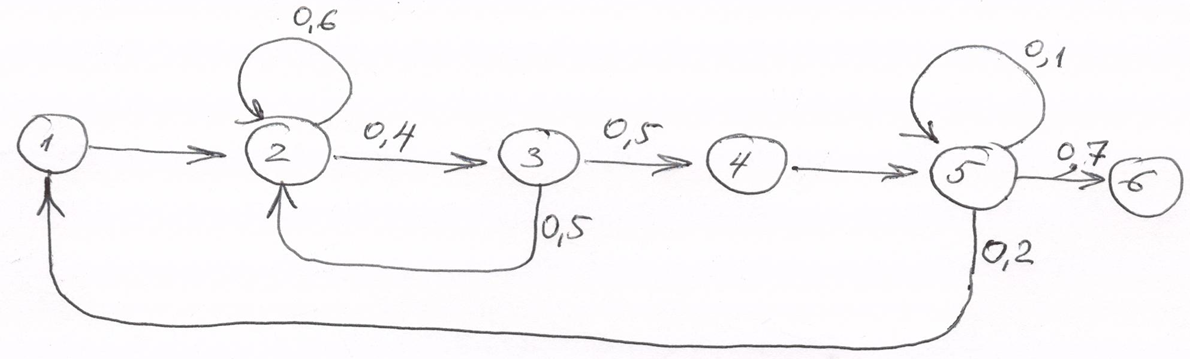
\includegraphics[width=.85\textwidth]{img/scheme_0}}
  \caption{Граф GERT-сети}
\end{figure}
\item Каждой дуге-работе ($ij$) поставлены в соответствие следующие данные:
\begin{enumerate}
\item Закон распределения времени выполнения работы. Будем считать его нормальным;
\item Параметры закона распределения (математическое ожидание \textbf{M} и дисперсия \textbf{D});
\item Вероятность $p_{ij}$ выполнения работы, показанная на графе.
\end{enumerate}
\end{enumerate}


\subsection{Задание}
\subsubsection{Часть 1}
Используя методику GERT, изложенную в книге «Методы анализа сетей»\\
Найти:
\begin{enumerate}
\item Вероятность выхода в завершающий узел графа (для всех вариантов узел 6);
\item Производящую функцию длительности процесса от начального узла  до завершающего узла;
\item Математическое ожидание длительности процесса от начального узла  до завершающего узла;
\item Дисперсию ожидание длительности процесса от начального узла  до завершающего узла;
\end{enumerate}
В отчете перечислить все петли всех порядков, обнаруженные на графе, выписать уравнение Мейсона, получить решение для $W_E(S)$ и найти требуемые параметры. Примерно так, как это сделано в примере на стр. 403–409 книги Филипса и Гарсиа «Методы анализа сетей»
\subsubsection{Часть 2}
Повторить пункты задания 2, 3, 4 используя методику анализа потокового графа, основанную на обработке матрицы передач (Branch Transmittance Matrix). 


Для выполнения задания рекомендуется пользоваться следующими источниками:
\begin{enumerate}
\item Филипс и Гарсиа «Методы анализа сетей»
\item Презентация GERT\_\&\_Flowgraph\_Algebra.pdf (выложена в ИНТРАНЕТ)
\item Ren\_The Methodology of Flowgraph.pdf
\end{enumerate}

\section{Решение}
\subsection{Часть 1}
Чтобы определить эквивалентную W-функцию для анализируемой GERT-сети, необходимо замкнуть сеть дугой, исходящей из узла 6 в узел 1 (рис. \ref{pic_1}).
\begin{figure}[H]
  \centering
  \fbox{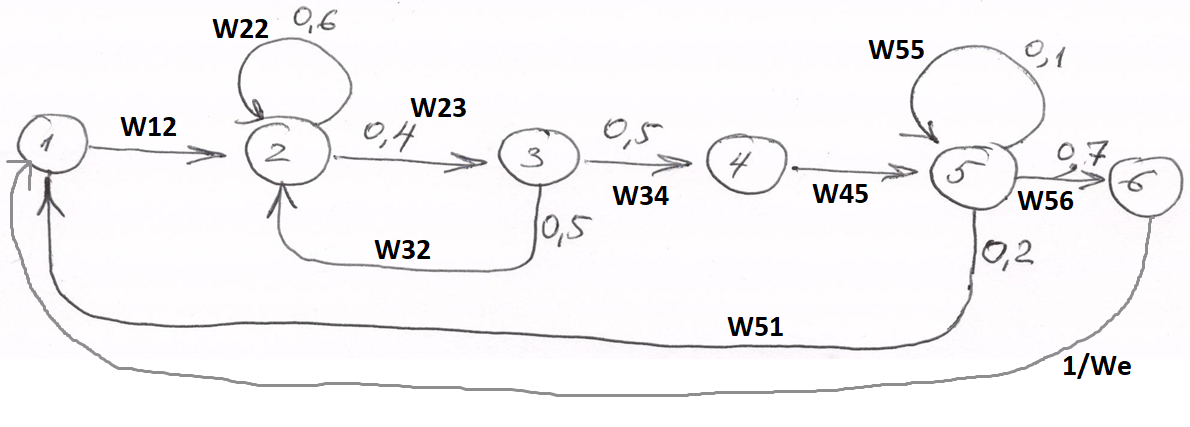
\includegraphics[width=\textwidth]{img/scheme_1}}
  \caption{Замкнутая GERT-сеть}
  \label{pic_1}
\end{figure}
Далее, выпишем в таблицу данные графа(мат. ожидание, дисперсия, W-функции)

\tabulinesep = 1mm
\begin{longtabu} to \textwidth {|X[8,c , m ] |X[8,c , m ] | X[15,l, m ]| X[15,l, m ]|X[15,l, m ]|X[25,l, m ]|}\firsthline\hline
\textbf{Начало}&\textbf{Конец}&\textbf{Вес ребра}&\textbf{Мат. ожидание}&\textbf{Дисперсия}&\textbf{W-функция}\\ \hline \endfirsthead
1	&2	&1	&20	&9	&$exp(20s+4.5s^2)$	\\ \hline
2	&2	&0.6&30	&16	&$0.6*exp(30s+8s^2)$	\\ \hline
2	&3	&0.4&40	&25	&$0.4*exp(40s+12.5s^2)$	\\ \hline
3	&2	&0.5&28	&16	&$0.5*exp(28s+8s^2)$	\\ \hline
3	&4	&0.5&37	&16	&$0.5*exp(37s+8s^2)$	\\ \hline
4	&5	&1	&30	&25	&$exp(30s+12.5s^2)$	\\ \hline
5	&1	&0.2&30	&16	&$0.2*exp(30s+8s^2)$	\\ \hline
5	&5	&0.1&10	&4	&$0.1*exp(10s+2s^2)$	\\ \hline
5	&6	&0.7&30	&16	&$0.7*exp(30s+8s^2)$	\\ \hline
\caption{Данные анализируемой GERT-сети}
\end{longtabu}
\textbf{Петли первого порядка:}
\begin{itemize}
\item $W_{12}W_{23}W_{34}W_{45}W_{51}$;
\item $W_{12}W_{23}W_{34}W_{45}W_{56}\frac{1}{W_e}$;
\item $W_{22}$;
\item $W_{23}W_{32}$;
\item $W_{55}$;
\end{itemize}
\textbf{Петли второго порядка:}
\begin{itemize}
\item $W_{22}W_{55}$;
\item $W_{55}W_{23}W_{32}$;
\end{itemize}
\textbf{Уравнение Мейсона}:
\begin{multline*}
H = 1 - W_{12}W_{23}W_{34}W_{45}W_{51} - W_{12}W_{23}W_{34}W_{45}W_{56}\frac{1}{W_e} - W_{22} - W_{23}W_{32} - W_{55}\\
 + W_{22}W_{55} + W_{55}W_{23}W_{32} = 0
\end{multline*}
\textbf{Выведем $W_E(S)$:}
\begin{equation*}
1 - W_{12}W_{23}W_{34}W_{45}W_{51} - W_{22} - W_{23}W_{32} - W_{55} + W_{22}W_{55} + W_{55}W_{23}W_{32} = W_{12}W_{23}W_{34}W_{45}W_{56}\frac{1}{W_e}
\end{equation*}
\begin{multline*}
W_E(S) =\\
(W_{12}W_{23}W_{34}W_{45}W_{56})/(1 - W_{12}W_{23}W_{34}W_{45}W_{51} - W_{22} - W_{23}W_{32} - W_{55} + W_{22}W_{55} + W_{55}W_{23}W_{32})
\end{multline*}

Вычислим математическое ожидание и дисперсию: $M_E(s) = 1$ при $s=0$

Так как $W_E(s)=p_E M_E (s)$,  то  $p_E=W_E(0)$, тогда $M_E(s)=\frac{W_E(s)}{p_E} =\frac{W_E(s)}{W_E(0)}$

Вычисляя первую и вторую производные по $s$ функции $M_E(s)$, и полагая $s=0$, находим математическое ожидание:
\begin{equation*}
\mu_{1E}=\frac{\partial M_E(s)}{\partial s}|s=0
\end{equation*}

и дисперсию:
\begin{equation*}
\sigma^2=\mu_{2E}-[\mu_{1E}]^2
\end{equation*}

Вероятность выхода в завершающий узел графа:
\begin{equation*}
p_E=W_E (0)
\end{equation*}
Был написан скрипт matlab.
\begin{lstlisting}[language={matlab}, caption={Код Matlab}]
clc
%Исходные данные
%М — математическое ожидание
%D — дисперсия
%P — вероятность
P12 = 1; M12 = 20; D12 = 9; 
P22 = 0.6; M22 = 30; D22 = 16; 
P23 = 0.4; M23 = 40; D23 = 25; 
P32 = 0.5; M32 = 28; D32 = 16; 
P34 = 0.5; M34 = 37; D34 = 16; 
P45 = 1; M45 = 30; D45 = 25; 
P51 = 0.2; M51 = 30; D51 = 16; 
P55 = 0.1; M55 = 10; D55 = 4; 
P56 = 0.7; M56 = 30; D56 = 16; 
 
syms s
%W функции
W12 = P12*exp(M12*s+D12/2*s^2);
W22 = P22*exp(M22*s+D22/2*s^2);
W23 = P23*exp(M23*s+D23/2*s^2);
W32 = P32*exp(M32*s+D32/2*s^2);
W34 = P34*exp(M34*s+D34/2*s^2);
W45 = P45*exp(M45*s+D45/2*s^2);
W51 = P51*exp(M51*s+D52/2*s^2);
W55 = P55*exp(M55*s+D55/2*s^2);
W56 = P56*exp(M56*s+D56/2*s^2);
 
We = (W12*W23*W34*W45*W56)/(1 — W12*W23*W34*W45*W51 — W22 — W23*W32 — W55+W22*W55+W55*W23*W32);
 
We = simplify(We)
We0 = subs(We, 's', 0)  % We(0)
 
% Нахождение мат. ожидания и дисперсии
Me = We/We0;
 
% Нахождение производной первого порядка при s=0
m1 = diff(Me, 's');     
m1 = subs(m1, 's', 0)   % Замена символа s на 0 в выражении m1
 
% Нахождение производной второго порядка при s=0
m2 = diff(Me, 's',2);
m2=subs(m2, 's', 0)     % Замена символа s на 0 в выражении m2
 
% Нахождение дисперсии времени выхода процесса в завершающий узел графа
D = m2 — (m1)^2
\end{lstlisting}
\begin{lstlisting}[language={matlab}, caption={Результат}, basicstyle=\ttfamily]
We =
-(7*exp((s*(91*s + 314))/2))/(5*exp(2*s*(s + 5)) - 3*exp(10*s*(s + 4)) + 30*exp(2*s*(4*s + 15)) - exp((3*s*(15*s + 52))/2) + 10*exp((s*(41*s + 136))/2) + 2*exp((s*(91*s + 314))/2) - 50)
 
We0 =
1
 
m1 =
2845/7
 
m2 =
11938987/49
 
D =
3844962/49
\end{lstlisting}
Были получены следующие результаты:
\begin{enumerate}
\item Вероятность выхода в завершающий узел графа равна 100\% ($p=W_E=1$).
\item Математическое ожидание 406,43.
\item Дисперсия времени выхода процесса в завершающий узел графа 78 468,61.
\end{enumerate}
\subsection{Часть 2}
Алгоритм дальнейших действий основан на:
\begin{itemize}
\item Презентация GERT\_\&\_Flowgraph\_Algebra.pdf (со слайда 56);
\item Ren\_The Methodology of Flowgraph.pdf (со страницы 35).
\end{itemize}
Определим матрицу Q, не забывая про обратную связь.
\begin{equation*}
Q = 
 \begin{pmatrix}
  0 & q_{12} & 0 & 0 & 0 & 0 \\
  0 & q_{22} & q_{23} & 0 & 0 & 0 \\ 
  0 & q_{32} & 0 & q_{34} & 0 & 0 \\ 
  0 & 0 & 0 & 0 & q_{45} & 0 \\ 
  q_{51} & 0 & 0 & 0 & q_{55} & q_{56} \\ 
  w_{61} & 0 & 0 & 0 & 0 & 0 
 \end{pmatrix}
\end{equation*}
Определим матрицу коэффициентов $A=I_6-Q^T$.
\begin{equation*}
A = 
 \begin{pmatrix}
    1&       0&    0&    0&    -q_{51}& -w_{61}\\
 -q_{12}& 1 - q_{22}& -q_{32}&    0&       0&    0\\
    0&    -q_{23}&    1&    0&       0&    0\\
    0&       0& -q_{34}&    1&       0&    0\\
    0&       0&    0& -q_{45}& 1 - q_{55}&    0\\
    0&       0&    0&    0&    -q_{56}&    1
 \end{pmatrix}
\end{equation*}
Находим 
\begin{equation*}
det(A)
\end{equation*}
далее
\begin{equation*}
\frac{\partial det(A)}{\partial w_{61}}
\end{equation*}
\begin{equation*}
det(A | w_{61}=0)
\end{equation*}
Далее можно вывести $W_E(S)$ с помощью формулы:
\begin{equation*}
W_E(S)=-\frac{\frac{\partial det(A)}{\partial w_{61}}}{det(A | w_{61}=0)}
\end{equation*}
Для расчетов, был написан matlab скрипт.
\begin{lstlisting}[language={matlab}, caption={Matlab скрипт}, basicstyle=\ttfamily]
clc; clearvars

syms q12
syms q22
syms q23
syms q32
syms q34
syms q45
syms q51
syms q55
syms q56
syms w61
syms s

Q=[0 q12 0 0 0 0;
   0 q22 q23 0 0 0;
   0 q32 0 q34 0 0;
   0 0 0 0 q45 0;
   q51 0 0 0 q55 q56;
   w61 0 0 0 0 0];

A1 = eye(size(Q,1)) - transpose(Q);
disp(A1);

det_A1 = det(A1);

det_dw=diff(det_A1, w61);

det2_A1=subs(det_A1, w61, 0);

We= -det_dw/det2_A1;
disp(We);
\end{lstlisting}
\begin{lstlisting}[language={matlab}, caption={Результат}, basicstyle=\ttfamily]
[    1,       0,    0,    0,    -q51, -w61]
[ -q12, 1 - q22, -q32,    0,       0,    0]
[    0,    -q23,    1,    0,       0,    0]
[    0,       0, -q34,    1,       0,    0]
[    0,       0,    0, -q45, 1 - q55,    0]
[    0,       0,    0,    0,    -q56,    1]
 
 
-(q12*q23*q34*q45*q56)/(q22 + q55 + q23*q32 - q22*q55 - q23*q32*q55 + q12*q23*q34*q45*q51 - 1)
\end{lstlisting}
Во второй строчке был получен $W_E(S)$, который полностью(за исключением знаков) совпадает с $W_E(S)$ найденным в части 1.

Далее, имея $W_E(S)$ находим необходимые переменные.
\begin{lstlisting}[language={matlab}, caption={Matlab скрипт}]
clc; clearvars

%М — математическое ожидание
%D — дисперсия
%P — вероятность
P12 = 1; M12 = 20; D12 = 9; 
P22 = 0.6; M22 = 30; D22 = 16; 
P23 = 0.4; M23 = 40; D23 = 25; 
P32 = 0.5; M32 = 28; D32 = 16; 
P34 = 0.5; M34 = 37; D34 = 16; 
P45 = 1; M45 = 30; D45 = 25; 
P51 = 0.2; M51 = 30; D51 = 16; 
P55 = 0.1; M55 = 10; D55 = 4; 
P56 = 0.7; M56 = 30; D56 = 16; 

syms q12
syms q22
syms q23
syms q32
syms q34
syms q45
syms q51
syms q55
syms q56
syms w61
syms s

Q=[0 q12 0 0 0 0;
   0 q22 q23 0 0 0;
   0 q32 0 q34 0 0;
   0 0 0 0 q45 0;
   q51 0 0 0 q55 q56;
   w61 0 0 0 0 0];

A1 = eye(size(Q,1)) - transpose(Q);
disp(A1);

det_A1 = det(A1);
disp(det_A1);

det_dw=diff(det_A1, w61);
disp(det_dw);

det2_A1=subs(det_A1, w61, 0);
disp(det2_A1);

We= -det_dw/det2_A1;
disp(We);


syms s

We=subs(We, q12, P12*exp(M12*s+D12/2*s^2));
We=subs(We, q22, P22*exp(M22*s+D22/2*s^2));
We=subs(We, q23, P23*exp(M23*s+D23/2*s^2));
We=subs(We, q32, P32*exp(M32*s+D32/2*s^2));
We=subs(We, q34, P34*exp(M34*s+D34/2*s^2));
We=subs(We, q45, P45*exp(M45*s+D45/2*s^2));
We=subs(We, q51, P51*exp(M51*s+D51/2*s^2));
We=subs(We, q55, P55*exp(M55*s+D55/2*s^2));
We=subs(We, q56, P56*exp(M56*s+D56/2*s^2));

We = simplify(We)
We0 = subs(We, 's', 0)  % We(0)
 
% Нахождение мат. ожидания и дисперсии
Me = We/We0;
 
% Нахождение производной 1-го порядка при s=0
m1 = diff(Me, 's');     
m1 = subs(m1, 's', 0)   % Замена символа s на 0 в выражении m1
 
% Нахождение производной 2-го порядка при s=0
m2 = diff(Me, 's',2);
m2=subs(m2, 's', 0)     % Замена символа s на 0 в выражении m2
 
% Нахождение дисперсии времени выхода процесса в завершающий узел графа
D = m2 - (m1)^2
\end{lstlisting}

\begin{lstlisting}[language={matlab}, caption={Результат}, basicstyle=\ttfamily]
We =
-(7*exp((s*(91*s + 314))/2))/(5*exp(2*s*(s + 5)) - 3*exp(10*s*(s + 4)) + 30*exp(2*s*(4*s + 15)) - exp((3*s*(15*s + 52))/2) + 10*exp((s*(41*s + 136))/2) + 2*exp((s*(91*s + 314))/2) - 50)
 
We0 =
1
 
m1 =
2845/7
 
m2 =
11938987/49
 
D =
3844962/49
\end{lstlisting}
Были получены следующие результаты:
\begin{enumerate}
\item Вероятность выхода в завершающий узел графа равна 100\% ($p=W_E=1$).
\item Математическое ожидание 406,43.
\item Дисперсия времени выхода процесса в завершающий узел графа 78 468,61.
\end{enumerate}
Которые полностью совпадает с результатами части 1.



%------------------------------------------------------------------------------

%\addcontentsline{toc}{section}{Список литературы}
%\bibliography{thesis}
%\bibliographystyle{ugost2008}

\end{document}